% Created 2022-12-30 Fri 17:49
\documentclass[9pt, b5paper]{article}
\usepackage{xeCJK}
\usepackage{minted}
\usepackage[T1]{fontenc}
\usepackage[scaled]{beraserif}
\usepackage[scaled]{berasans}
\usepackage[scaled]{beramono}
\usepackage{graphicx}
\usepackage{xcolor}
\usepackage{multirow}
\usepackage{multicol}
\usepackage{float}
\usepackage{textcomp}
\usepackage{algorithm}
\usepackage{algorithmic}
\usepackage{latexsym}
\usepackage{natbib}
\usepackage{geometry}
\geometry{left=1.2cm,right=1.2cm,top=1.5cm,bottom=1.2cm}
\newminted{common-lisp}{fontsize=\footnotesize} 
\usepackage[xetex,colorlinks=true,CJKbookmarks=true,linkcolor=blue,urlcolor=blue,menucolor=blue]{hyperref}
\author{deepwaterooo}
\date{\today}
\title{游戏通用功能底层逻辑Android SDK 封装}
\hypersetup{
  pdfkeywords={},
  pdfsubject={},
  pdfcreator={Emacs 27.2 (Org mode 8.2.7c)}}
\begin{document}

\maketitle
\tableofcontents


\section{Android SDK 封装for unity games}
\label{sec-1}
\begin{itemize}
\item 现在的流程前几天早就已经走通了.那么现在可以简单实现的就是安卓SDK中的登录界面.但是因为游戏热更新服务器还没有搭建起来,现有登录界面也可以凑合,没太多热情去弄登录界面
\item 另一个界面可以是游戏过程中的音量控制.两种思路:
\begin{itemize}
\item\relax [ \textbf{重点需求} ]:当用户按了手机上的音量调节,是需要游戏注册广播,能够监听到音量调节变化,并自动调出音量调节窗口的 [调不调出来呢?可以不用,因为安卓系统自己配备的有]
\item\relax [ \textbf{重点需求} ] 相反方向上的,同样的,当用户通过安卓SDK 或是游戏界面来调控音量的时候,也要能够操作成功,比如滑动条滑动手势调节音量
\item 可以把视图界面也包装在安卓SDK中,但是会显得比较复杂.搜到两种不同的实现,一个简单一个复杂一点儿,但两个都没有注册监听系统音量变化,要自己实现(就写一个自己的广播接收器来接收系统音量变化广播就可以了,主要是安卓视图界面做起来比较麻烦)
\begin{itemize}
\item 但是安卓SDK 中实现这些所有的功能是最简单的思路,只是个人不喜欢操作视图而已
\item \url{https://blog.csdn.net/zhaokaiqiang1992/article/details/34441229?spm=1001.2101.3001.6650.6&utm_medium=distribute.pc_relevant.none-task-blog-2\%7Edefault\%7EESLANDING\%7Edefault-6-34441229-blog-10644497.pc_relevant_landingrelevant&depth_1-utm_source=distribute.pc_relevant.none-task-blog-2\%7Edefault\%7EESLANDING\%7Edefault-6-34441229-blog-10644497.pc_relevant_landingrelevant&utm_relevant_index=6} 这个界面简单也难看一点儿
\item \url{https://blog.csdn.net/cf8833/article/details/89360609} 这个实现复杂一点儿,但好像比较好看
\item 这个思路设计实现起来都是最简单的,麻烦的是视图界面,最主要的是上面两个例子中都没有带需要的图片,得自己找图片配或是找其它类似的例子
\end{itemize}
\item 游戏引擎做界面会容易很多,可以从安卓SDK中拿安卓平台原生数据,反馈到unity游戏界面上来实现 来更为简单方便. 这是现有的三个例子里面最为简单的一个,因为视图界面由游戏引擎来做(我也已经做好了) 
\begin{itemize}
\item 参照这个例子来实现好了: \url{https://codeantenna.com/a/73H89XeBeL}
\item 上面的例子中最主要缺陷是通过接口的形式将接收到的系统广播传给游戏端,与自己现有层次的模块化设计不符,会影响代码的移植和复用. 这个接口的例子本身的回调没有问题,可以连通
\item 可以参考这个自定义广播接收器的办法,多加一个类在.jar安卓包中,实现从游戏端动态注册安卓广播: 最先测试这个思路的两篇网页想法
\begin{itemize}
\item \url{https://blog.csdn.net/yhx956058885/article/details/110949067}
\end{itemize}
\end{itemize}
\end{itemize}

\item 视图摆游戏端的上面的两个思路: 想比于安卓SDK中完全实现视图和回调要难,因为涉及到两者的交互与适配.会把两的原理都弄懂
\begin{itemize}
\item 接口例子中最主要缺陷是通过接口的形式将接收到的系统广播传给游戏端,与自己现有层次的模块化设计不符,会影响代码的移植和复用. 这个接口的例子本身的回调没有问题,可以连通
\item 游戏端动态注册安卓广播的,我哪里写得不对,想要再调试测试一下,    
\item 另接口回调的思路中:
\item 现在的问题是,游戏热 \textbf{更新程序域里没有连接好音量滑动条的手势检测与触摸事件},需要把这个连通.因为当游戏中了这个视图,为的就是视图比硬件操作方便,如果这个功能没有实现或是连通,用户体验会变差.会把这个功能连通
\end{itemize}
\end{itemize}

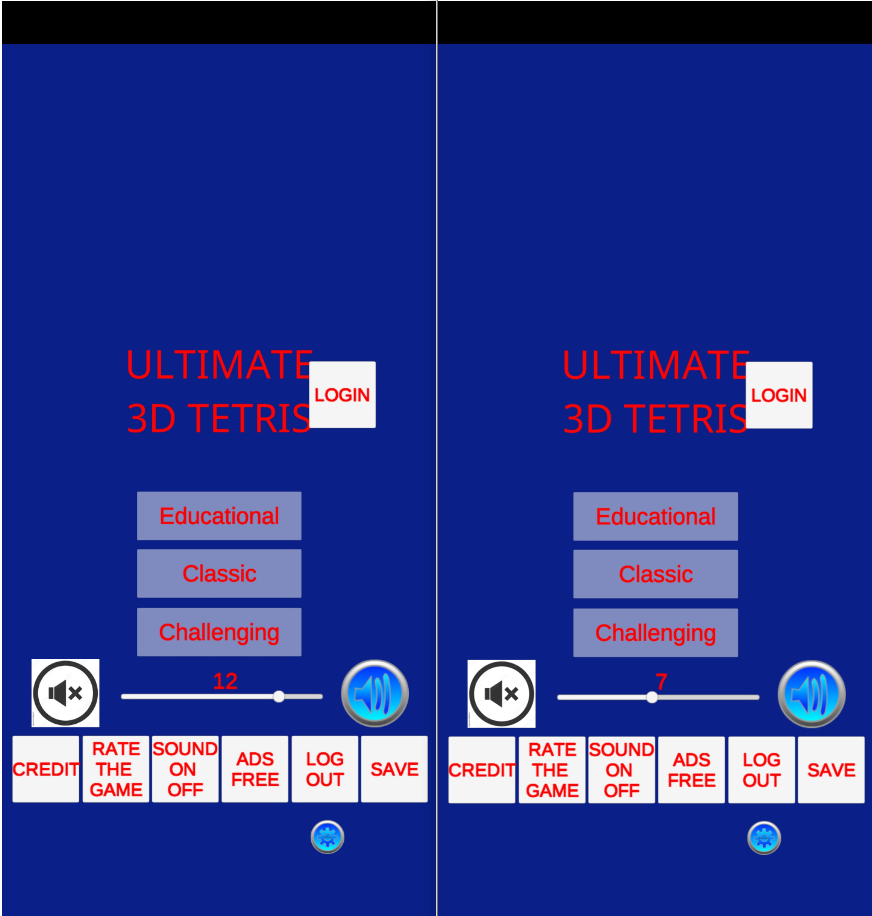
\includegraphics[width=.9\linewidth]{./pic/readme_20221230_174540.png}
\begin{itemize}
\item Initial design, to be modified and linked later
\item Will work on packing lower layer Android SDK feature/functionality packing for coming a few days
\item 屏幕适配可需要再改一下
\end{itemize}

\section{Unity安卓共享纹理}
\label{sec-2}
\begin{itemize}
\item 之前一直有想法:就是把游戏中所用到的平移(四个按钮)与旋转(六个按钮)做成安卓原生开发,做成透明,与游戏端画面叠加绘制
\begin{itemize}
\item 原本也可以不用,前提是我能够在游戏端将这两块画面做得漂亮
\item 自己做不漂亮的时候,就去想,能不能从安卓端原生画出来,毕竟画出来的刻度会是精准的,并将十个按钮设置为半透明,达到精准完美的程度
\end{itemize}
\item 现在看,这些实现起来都是有理论支撑,可以做到的,参考的github项目也已经被我fork到自己的了
\item 等安卓SDK接完,可能会试一下自己游戏中能够实现这些
\item 一些基础原理: 参考网页: \url{https://blog.csdn.net/jnlws/article/details/113176253}
\begin{itemize}
\item 其实还可参考的包括:
\begin{itemize}
\item \url{https://github.com/littlesome/UnityTransparent}
\item \url{https://juejin.cn/post/6986252493541867533} 
\end{itemize}
\end{itemize}
\end{itemize}
\begin{minted}[fontsize=\scriptsize,linenos=false]{java}
public class GLTexture {
    private static final String TAG = "GLTexture";

    private static final String imageFilePath = "/sdcard/1Atest/image.jpg";

    private int mTextureID = 0;
    private int mTextureWidth = 0;
    private int mTextureHeight = 0;

    SurfaceTexture mCameraInputSurface;
    SurfaceTexture mOutputSurfaceTexture;
    int mOutputTex[];

// OpenGL 渲染的上下文及配置: 多线程安全(安卓 游戏)
    private volatile EGLContext mSharedEglContext;
    private volatile EGLConfig mSharedEglConfig;

    private EGLDisplay mEGLDisplay;
    private EGLContext mEglContext;
    private EGLSurface mEglSurface;

    // 创建单线程池,用于处理OpenGL纹理
    private final ExecutorService mRenderThread = Executors.newSingleThreadExecutor();
    // 使用Unity线程Looper的Handler,用于执行Java层的OpenGL操作
    private Handler mUnityRenderHandler;

    public GLTexture() { }
    public int getStreamTextureWidth() {
        //Log.d(TAG,"mTextureWidth = "+ mTextureWidth);
        return mTextureWidth;
    }
    public int getStreamTextureHeight() {
        //Log.d(TAG,"mTextureHeight = "+ mTextureHeight);
        return mTextureHeight;
    }
    public int getStreamTextureID() {
        Log.d(TAG,"getStreamTextureID sucess = "+ mTextureID);
        return mTextureID;
    }
    private void glLogE(String msg) {
        Log.e(TAG, msg + ", err=" + GLES20.glGetError());
    }

    // 被unity调用
    public void setupOpenGL() {
        Log.d(TAG, "setupOpenGL called by Unity ");

        // 注意:该调用一定是从Unity绘制线程发起
        if (Looper.myLooper() == null) {
            Looper.prepare();
        }
        mUnityRenderHandler = new Handler(Looper.myLooper());

        // Unity获取EGLContext
        mSharedEglContext = EGL14.eglGetCurrentContext();
        if (mSharedEglContext == EGL14.EGL_NO_CONTEXT) {
            glLogE("eglGetCurrentContext failed");
            return;
        }
        glLogE("eglGetCurrentContext success");

        EGLDisplay sharedEglDisplay = EGL14.eglGetCurrentDisplay();
        if (sharedEglDisplay == EGL14.EGL_NO_DISPLAY) {
            glLogE("sharedEglDisplay failed");
            return;
        }
        glLogE("sharedEglDisplay success");

        // 获取Unity绘制线程的EGLConfig
        int[] numEglConfigs = new int[1];
        EGLConfig[] eglConfigs = new EGLConfig[1];
        if (!EGL14.eglGetConfigs(sharedEglDisplay, eglConfigs, 0, eglConfigs.length,
                                 numEglConfigs, 0)) {
            glLogE("eglGetConfigs failed");
            return;
        }
        mSharedEglConfig = eglConfigs[0];
        mRenderThread.execute(new Runnable() {
                @Override
                public void run() {
                    // 初始化OpenGL环境
                    initOpenGL();
                    // 生成OpenGL纹理ID
                    int textures[] = new int[1];
                    GLES20.glGenTextures(1, textures, 0);
                    if (textures[0] == 0) { glLogE("glGenTextures failed"); return; }
                    else { glLogE("glGenTextures success"); }
                    mTextureID = textures[0];
                    mTextureWidth = 670;
                    mTextureHeight = 670;
                }
            });
    }
    private void initOpenGL() {
        mEGLDisplay = EGL14.eglGetDisplay(EGL14.EGL_DEFAULT_DISPLAY);
        if (mEGLDisplay == EGL14.EGL_NO_DISPLAY) {
            glLogE("eglGetDisplay failed");
            return;
        }
        glLogE("eglGetDisplay success");

        int[] version = new int[2];
        if (!EGL14.eglInitialize(mEGLDisplay, version, 0, version, 1)) {
            mEGLDisplay = null;
            glLogE("eglInitialize failed");
            return;
        }
        glLogE("eglInitialize success");

        int[] eglContextAttribList = new int[]{
            EGL14.EGL_CONTEXT_CLIENT_VERSION, 3, // 该值需与Unity绘制线程使用的一致
            EGL14.EGL_NONE
        };
        // 创建Java线程的EGLContext时,将Unity线程的EGLContext和EGLConfig作为参数传递给eglCreateContext,
        // 从而实现两个线程共享EGLContext
        mEglContext = EGL14.eglCreateContext(mEGLDisplay, mSharedEglConfig, mSharedEglContext,
                                             eglContextAttribList, 0);
        if (mEglContext == EGL14.EGL_NO_CONTEXT) {
            glLogE("eglCreateContext failed");
            return;
        }
        glLogE("eglCreateContext success");

        int[] surfaceAttribList = {
            EGL14.EGL_WIDTH, 64,
            EGL14.EGL_HEIGHT, 64,
            EGL14.EGL_NONE
        };
        // Java线程不进行实际绘制,因此创建PbufferSurface而非WindowSurface
        // 创建Java线程的EGLSurface时,将Unity线程的EGLConfig作为参数传递给eglCreatePbufferSurface
        mEglSurface = EGL14.eglCreatePbufferSurface(mEGLDisplay, mSharedEglConfig, surfaceAttribList, 0);
        if (mEglSurface == EGL14.EGL_NO_SURFACE) {
            glLogE("eglCreatePbufferSurface failed");
            return;
        }
        glLogE("eglCreatePbufferSurface success");

        if (!EGL14.eglMakeCurrent(mEGLDisplay, mEglSurface, mEglSurface, mEglContext)) {
            glLogE("eglMakeCurrent failed");
            return;
        }
        glLogE("eglMakeCurrent success");

        GLES20.glFlush();
    }
    public void updateTexture() {
        // Log.d(TAG,"updateTexture called by unity");
        mRenderThread.execute(new Runnable() {
                @Override
                public void run() {
                    final Bitmap bitmap = BitmapFactory.decodeFile(imageFilePath);
//                if(bitmap == null)
//                    Log.d(TAG,"bitmap decode faild" + bitmap);
//                else
//                    Log.d(TAG,"bitmap decode success" + bitmap);
                    mUnityRenderHandler.post(new Runnable() {
                            @Override
                            public void run() {
                                GLES20.glBindTexture(GLES20.GL_TEXTURE_2D, mTextureID);
                                GLES20.glTexParameteri(GLES11Ext.GL_TEXTURE_EXTERNAL_OES, GLES20.GL_TEXTURE_MIN_FILTER, GLES20.GL_NEAREST);
                                GLES20.glTexParameteri(GLES11Ext.GL_TEXTURE_EXTERNAL_OES, GLES20.GL_TEXTURE_MAG_FILTER, GLES20.GL_NEAREST);
                                GLES20.glTexParameteri(GLES20.GL_TEXTURE_2D, GLES20.GL_TEXTURE_WRAP_S, GLES20.GL_CLAMP_TO_EDGE);
                                GLES20.glTexParameteri(GLES20.GL_TEXTURE_2D, GLES20.GL_TEXTURE_WRAP_T, GLES20.GL_CLAMP_TO_EDGE);
                                GLES20.glTexParameteri(GLES20.GL_TEXTURE_2D, GLES20.GL_TEXTURE_MAG_FILTER, GLES20.GL_LINEAR);
                                GLES20.glTexParameteri(GLES20.GL_TEXTURE_2D, GLES20.GL_TEXTURE_MIN_FILTER, GLES20.GL_LINEAR);
                                GLUtils.texImage2D(GLES20.GL_TEXTURE_2D, 0, bitmap, 0);
                                GLES20.glBindTexture(GLES20.GL_TEXTURE_2D, 0);
                                bitmap.recycle();
                            }
                        });
                }
            });
    }
    public void destroy() {
        mRenderThread.shutdownNow();
    }
}
\end{minted}
% Emacs 27.2 (Org mode 8.2.7c)
\end{document}